\newday{04 March 2024}
	\action{
		After seeing that with 1 datapoint the model does not learn I decide to make some simpler tests, I will train a model that from a 19 element array predicts images with 2 channels and see if the input is too small for the model to predict anything. Three experiments will be performed:
		\begin{itemize}
			\item From a 19 elements array to a 2x128x128 image
			\item From a 19 elements array to a 2x64x64 image
			\item From a 19 elements array to a 2x32x32 image
		\end{itemize}
	}
	\rule{0.5\textwidth}{0.5pt}\\

	{\large \textbf{EXPERIMENT FromArrayToImage128-1}}\\
	
	{\normalsize HYPERPARAMETERS:}
	\begin{lstlisting}	
	*ARCHITECTURE HYPERPARAMETERS:
		-Fully Connected
		-Input shape: 19
		-Output shape: 32768
		-Hidden layers: [128, 128, 128, 128, 256, 256, 512, 2000, 4000]
		-Regularizer: None
		-Hidden Layers Activation: relu
		-Output Layer Activation: linear
		-Batch Normalization: False
		-Dropout: False, 0.2
	
	*COMPILATION HYPERPARAMETERS:
		-Optimizer: ADAM lr=0.001, beta_1=0.9, beta_2=0.999
		-Loss Function: MSE
		-Metric: MSE
	
	*TRAINING HYPERPARAMETERS:
		-Epochs: 10000
		-Batch size: 1
		-Callbacks: 
			-ReduceLROnPlateau: MSE 10 x0.1
			-Early Stop: MSE 25
	\end{lstlisting}
	
	{\normalsize VISUALIZATION:}
	\begin{lstlisting}
	*RESULTS:
        -Train MSE: 0.00010900569031946361
	\end{lstlisting}
	
	\begin{figure*}[ht!]
		\subfloat[Training Evolution]{%
		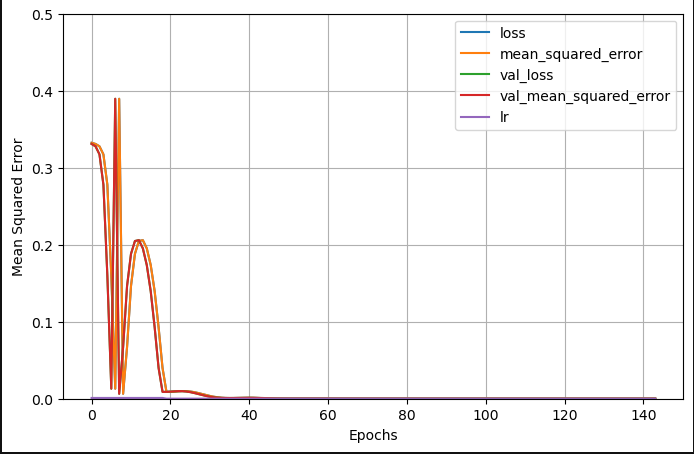
\includegraphics[ width=0.31\textwidth]{psf-FromArrayToImage128-1-evolution.png}}
		\hspace{\fill}
		\subfloat[Train example]{%
		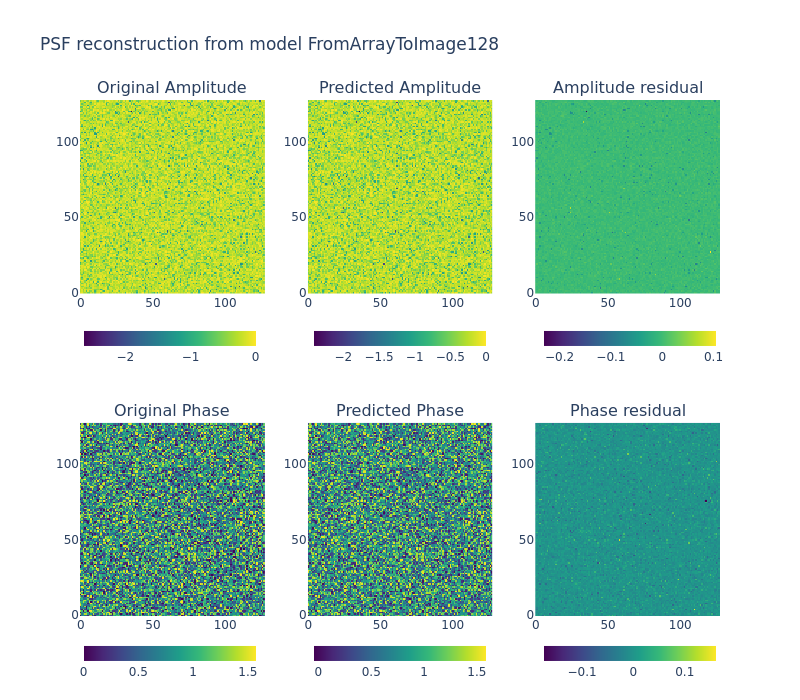
\includegraphics[ width=0.31\textwidth]{psf-FromArrayToImage128-1-train.png}}
		\hspace{\fill}
		\subfloat[Train example]{%
		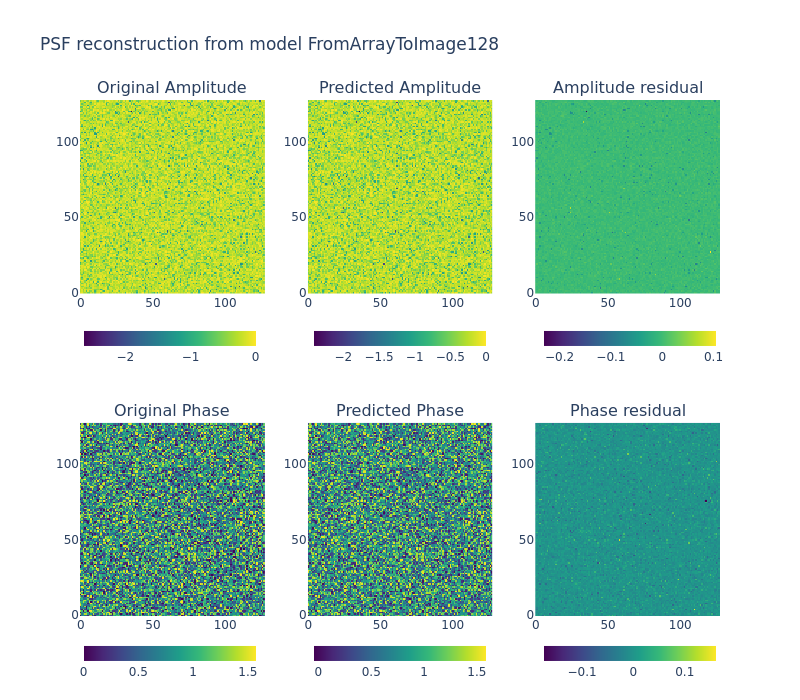
\includegraphics[ width=0.31\textwidth]{psf-FromArrayToImage128-1-train.png}}\\
		\caption{Results of training the model FromArrayToImage128-1}
	\end{figure*}
	
\FloatBarrier	
\rule{0.5\textwidth}{0.5pt}\\
	\action{
		From the previous experiment it is clear that a 19 element array as input is enough to reconstruct a random image of 2x128x128 resolution, what is happening for the psf reconstruction?.\\
		
		I will perform the other 2 stated experiments because it is quite fast.
	}
	\rule{0.5\textwidth}{0.5pt}\\

	{\large \textbf{EXPERIMENT •}}\\
	
	{\normalsize HYPERPARAMETERS:}
	\begin{lstlisting}	
	•
	\end{lstlisting}
	
	{\normalsize VISUALIZATION:}
	\begin{lstlisting}
	•
	\end{lstlisting}
	
	\begin{figure*}[ht!]
		\subfloat[Training Evolution]{%
		\includegraphics[ width=0.31\textwidth]{•-evolution.png}}
		\hspace{\fill}
		\subfloat[Validation example]{%
		\includegraphics[ width=0.31\textwidth]{•-val.png}}
		\hspace{\fill}
		\subfloat[Train example]{%
		\includegraphics[ width=0.31\textwidth]{•-train.png}}\\
		\caption{Results of training the model •}
	\end{figure*}
	
\FloatBarrier	
\rule{0.5\textwidth}{0.5pt}\\
	\rule{0.5\textwidth}{0.5pt}\\

	{\large \textbf{EXPERIMENT •}}\\
	
	{\normalsize HYPERPARAMETERS:}
	\begin{lstlisting}	
	•
	\end{lstlisting}
	
	{\normalsize VISUALIZATION:}
	\begin{lstlisting}
	•
	\end{lstlisting}
	
	\begin{figure*}[ht!]
		\subfloat[Training Evolution]{%
		\includegraphics[ width=0.31\textwidth]{•-evolution.png}}
		\hspace{\fill}
		\subfloat[Validation example]{%
		\includegraphics[ width=0.31\textwidth]{•-val.png}}
		\hspace{\fill}
		\subfloat[Train example]{%
		\includegraphics[ width=0.31\textwidth]{•-train.png}}\\
		\caption{Results of training the model •}
	\end{figure*}
	
\FloatBarrier	
\rule{0.5\textwidth}{0.5pt}\\
	\action{
		The results are satisfactory, I am going to try the exact same configuration for one data point of the PSF dataset and see what happens	
	}
	\rule{0.5\textwidth}{0.5pt}\\

	{\large \textbf{EXPERIMENT TestWith1DataPoint-3}}\\
	
	{\normalsize HYPERPARAMETERS:}
	\begin{lstlisting}
	*ARCHITECTURE HYPERPARAMETERS:
		-Fully Connected
		-Input shape: 19
		-Output shape: 32768
		-Hidden layers: [128, 128, 128, 128, 256, 256, 512, 2000, 4000]
		-Regularizer: None
		-Hidden Layers Activation: relu
		-Output Layer Activation: linear
		-Batch Normalization: False
		-Dropout: False, 0.2
	
	*COMPILATION HYPERPARAMETERS:
		-Optimizer: ADAM lr=0.001, beta_1=0.9, beta_2=0.999
		-Loss Function: MSE
		-Metric: MSE
	
	*TRAINING HYPERPARAMETERS:
		-Epochs: 10000
		-Batch size: 1
		-Callbacks: 
			-ReduceLROnPlateau: MSE 10 x0.1
			-Early Stop: MSE 25
	\end{lstlisting}
	
	{\normalsize VISUALIZATION:}
	\begin{lstlisting}
	*RESULTS:
        -Train MSE: 1.2409615010255948e-05
	\end{lstlisting}
	
	\begin{figure*}[ht!]
		\subfloat[Training Evolution]{%
		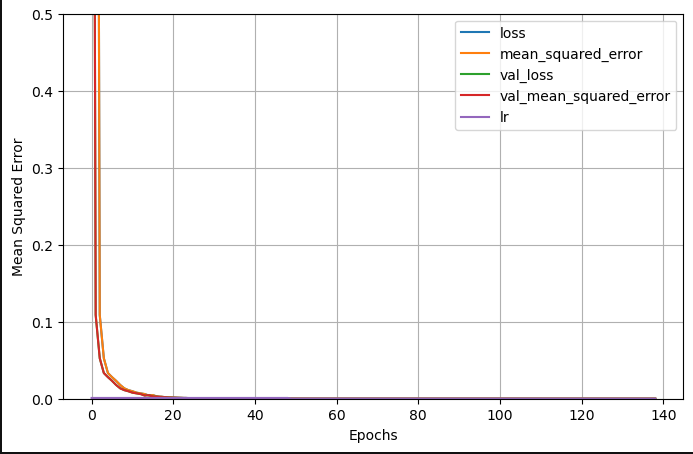
\includegraphics[ width=0.31\textwidth]{psf-TestWith1DataPoint-3-evolution.png}}
		\hspace{\fill}
		\subfloat[Train datapoint]{%
		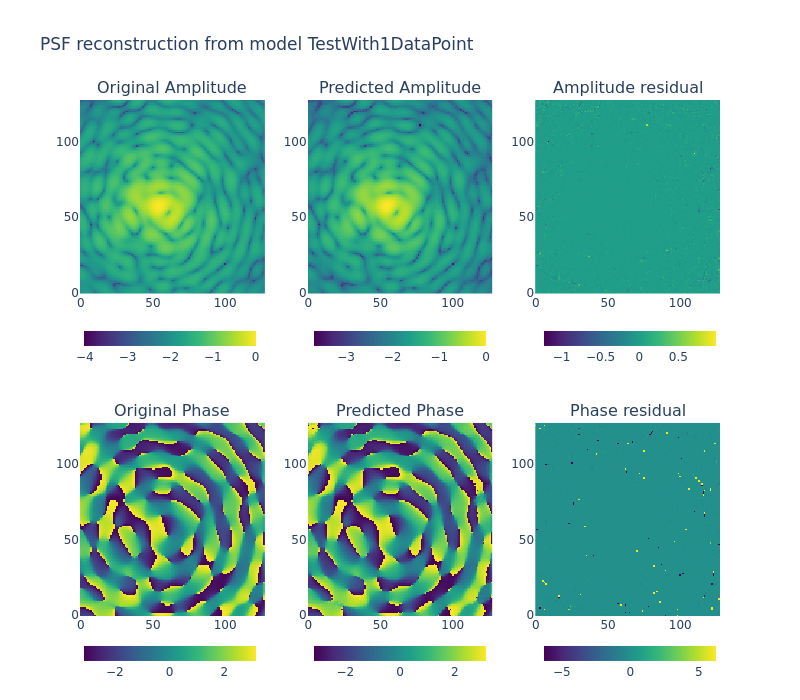
\includegraphics[ width=0.31\textwidth]{psf-TestWith1DataPoint-3-train.png}}
		\hspace{\fill}	
		\subfloat[Train datapoint]{%
		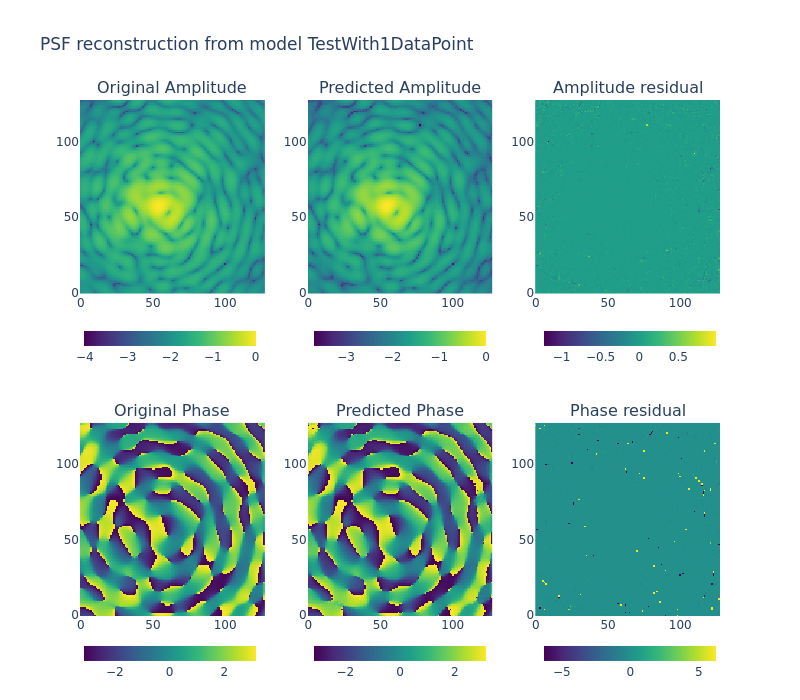
\includegraphics[ width=0.31\textwidth]{psf-TestWith1DataPoint-3-train.png}}\\
		\caption{Results of training the model TestWith1DataPoint-3}
	\end{figure*}
	
\FloatBarrier	
\rule{0.5\textwidth}{0.5pt}\\
	\action{
		The result has improved incredibly compared to the TestWith1DataPoint-1 and TestWith1DataPoint-2. The only difference I can see are the learning rates and the batch size. I will perform a series of experiments varying with batch size.
	}
\finishday